% ============================================================================
%  Hospital Management System — Project Report
%  Modelled on the Library Management System report (KU, Dept. of CSE).
%
%  Compiles with pdfLaTeX (Overleaf: just press Recompile).
%  Diagrams are drawn in TikZ so no external image files are required.
%  Screenshots are shown as labelled placeholder frames — replace each
%  \screenshot{...} with \includegraphics{yourfile} when you add real images.
%
%  TODO before subm&itting: confirm the items marked  % <-- VERIFY
% ============================================================================
\documentclass[12pt,a4paper]{report}

\usepackage[utf8]{inputenc}
\usepackage[T1]{fontenc}
\usepackage{lmodern}
\usepackage[margin=1in]{geometry}
\usepackage{graphicx}
\usepackage{setspace}
\usepackage{titlesec}
\usepackage{enumitem}
\usepackage{booktabs}
\usepackage{longtable}
\usepackage{array}
\usepackage{xcolor}
\usepackage{listings}
\usepackage{algorithm}
\usepackage{algpseudocode}
\usepackage{tikz}
\usepackage{pgfgantt}
\usepackage{caption}
\usepackage[hidelinks]{hyperref}

\usetikzlibrary{shapes.geometric, arrows.meta, positioning, fit, backgrounds, calc}

\onehalfspacing

% ---- Code listing style ----------------------------------------------------
\definecolor{codegray}{gray}{0.95}
\definecolor{codegreen}{rgb}{0.0,0.5,0.0}
\definecolor{codeblue}{rgb}{0.1,0.2,0.7}
\lstset{
  basicstyle=\ttfamily\footnotesize,
  backgroundcolor=\color{codegray},
  keywordstyle=\color{codeblue}\bfseries,
  commentstyle=\color{codegreen}\itshape,
  stringstyle=\color{purple},
  numbers=left, numberstyle=\tiny, numbersep=6pt,
  breaklines=true, showstringspaces=false, frame=single,
  tabsize=2, captionpos=b,
}

% ---- Screenshot placeholder helper ----------------------------------------
% Renders a framed grey box in place of a screenshot you will add later.
\newcommand{\screenshot}[1]{%
  \begin{center}
  \fbox{\begin{minipage}[c][4.2cm][c]{0.82\textwidth}
    \centering \itshape\color{gray} [ Screenshot placeholder — insert image here ]\\[4pt]
    \normalfont\small #1
  \end{minipage}}
  \end{center}}

% ---- Real screenshot figure: \rfig{file}{caption}{label} -------------------
\newcommand{\rfig}[3]{%
  \begin{figure}[htbp]
  \centering
  \fbox{\includegraphics[width=0.9\textwidth]{#1}}
  \caption{#2}\label{#3}
  \end{figure}}

% TikZ node styles reused across flowcharts
\tikzset{
  startstop/.style={rectangle, rounded corners, draw=black, fill=green!12, minimum width=2.6cm, minimum height=0.8cm, align=center},
  process/.style={rectangle, draw=black, fill=blue!8, minimum width=3.2cm, minimum height=0.8cm, align=center},
  decision/.style={diamond, aspect=2, draw=black, fill=orange!15, minimum width=2.8cm, align=center, inner sep=1pt},
  io/.style={trapezium, trapezium left angle=70, trapezium right angle=110, draw=black, fill=yellow!15, minimum width=2.6cm, minimum height=0.7cm, align=center},
  arrow/.style={-{Stealth[length=2mm]}, thick},
}

\begin{document}

% ===========================================================================
% TITLE PAGE
% ===========================================================================
\begin{titlepage}
\centering

\includegraphics[width=2.8cm]{pica/logo.png}\par
\vspace{12pt}
{\Large\bfseries Kathmandu University\par}
\vspace{2pt}
{\large Department of Computer Science and Engineering\par}
{\large Dhulikhel, Kavre\par}
\vspace{1.8cm}
{\large A Project Report\par}
\vspace{4pt}
{\large on\par}
\vspace{10pt}
{\LARGE\bfseries ``Hospital Management System''\par}
\vspace{10pt}
{\large [Code No.: COMP 207]\par}                              % <-- VERIFY course code
\vspace{6pt}
{\normalsize (For partial fulfillment of Year II / Semester II in Computer Science)\par}
\vspace{1.8cm}
{\large\bfseries Submitted by\par}
\vspace{6pt}
{\normalsize
Aayush Aacharya (Roll no. 1)\\
Aayush Adhikari (Roll no. 2)\\
Aarjan Adhikari (Roll no. 3)\\
Krish Ghimire (Roll no. 24)\\
 }                                    % <-- VERIFY names / roll numbers
\vspace{1.0cm}
{\large\bfseries Submitted to\par}
\vspace{2pt}
{\normalsize Dr. Rabindra Bista\\                                   % <-- VERIFY
Department of Computer Science and Engineering\par}
\vspace{1.6cm}
{\normalsize \today\par}                                       % <-- VERIFY submission date
\end{titlepage}

% ===========================================================================
% BONA FIDE CERTIFICATE
% ===========================================================================
\pagenumbering{roman}
\chapter*{Bona fide Certificate}
\thispagestyle{plain}
\vspace{0.5cm}
\begin{center}
This project work on\\[4pt]
{\bfseries ``Hospital Management System''}\\[4pt]
is the bona fide work of\\[6pt]
\emph{Aayush Aacharya (Roll no. 1), Aayush Adhikari (Roll no. 2),\\
Krish Ghimire (Roll no. 24), Aarjan Adhikarii (Roll no. 3)}\\[6pt]
who carried out the project work under my supervision.
\end{center}
\vspace{2.5cm}
\noindent
Project Supervisor\\[2pt]
\rule{6cm}{0.4pt}\\
Dr. Rabindra Bista\\                                              % <-- VERIFY supervisor
Lecturer\\
Department of Computer Science and Engineering

% ===========================================================================
% ACKNOWLEDGEMENTS
% ===========================================================================
\chapter*{Acknowledgements}
\addcontentsline{toc}{chapter}{Acknowledgements}
We express our sincere gratitude to all who contributed to the successful completion
of this project.

First, we would like to thank our project supervisor for their valuable guidance,
continuous support, and constructive feedback throughout the development of this
project. Their insights and encouragement played a crucial role in shaping both the
technical and conceptual aspects of our work.

We are also grateful to the faculty members of our department for providing the
necessary resources and academic environment that supported our learning and
project development.

We would like to acknowledge our teammates for their cooperation, dedication, and
collaborative efforts. Working together as a team helped us overcome challenges and
successfully implement the project objectives.

Finally, we extend our gratitude to our friends and family for their constant
encouragement and moral support throughout the course of this project.

% ===========================================================================
% ABSTRACT
% ===========================================================================
\chapter*{Abstract}
\addcontentsline{toc}{chapter}{Abstract}
The growing complexity of healthcare delivery has increased the need for efficient,
secure, and integrated hospital information systems. This project presents the design
and development of a web-based \textbf{Hospital Management System (HMS)} that
automates core clinical and administrative operations and connects the different
people involved in patient care through a single platform. The system provides secure
user authentication using \textbf{JSON Web Tokens (JWT)} with refresh-token rotation,
and implements \textbf{role-based access control} across five distinct roles---patient,
doctor, pharmacist, lab assistant, and administrator---so that each user interacts only
with the features appropriate to them. Patients can register, book and manage
appointments, view prescriptions and lab results, and settle bills; doctors manage
their availability, consult patients, issue prescriptions, order lab tests, and refer
patients to colleagues; lab assistants process test requests; pharmacists manage a
location-aware medicine inventory; and administrators manage staff, billing, rooms,
and system-wide records. The application is built using \textbf{React} with
\textbf{Tailwind CSS} on the frontend, and a \textbf{Node.js} and \textbf{Express}
backend integrated with a \textbf{MySQL} relational database through the
\textbf{Sequelize} ORM. Beyond in-application alerts, the system delivers
\textbf{outbound email and SMS notifications}, along with password-reset and
email-verification flows, so that patients stay informed without needing to log in. By
reducing manual paperwork, preventing double-booking, and centralising clinical
records, the proposed system improves the efficiency and reliability of hospital
operations and provides a robust foundation for future enhancements.

\vspace{0.4cm}
\noindent\textbf{Keywords:} Hospital Management System, React, Node.js, Express,
MySQL, Sequelize, JWT Authentication, Role-Based Access Control, RESTful API,
Full-Stack Development.

% ===========================================================================
% TABLE OF CONTENTS / FIGURES / TABLES
% ===========================================================================
\tableofcontents
\listoffigures
\listoftables

% ===========================================================================
\clearpage
\pagenumbering{arabic}

% ===========================================================================
% CHAPTER 1 — INTRODUCTION
% ===========================================================================
\chapter{Introduction}
Hospitals coordinate a large amount of information every day: patient records,
appointments, prescriptions, laboratory tests, billing, and pharmacy stock. When these
are handled manually or through disconnected tools, the result is duplicated effort,
long waiting times, lost records, and a higher chance of error. The adoption of
integrated digital systems has become essential to improve accuracy, accessibility, and
overall efficiency of healthcare delivery.

This project focuses on the development of a \textbf{Hospital Management System (HMS)}
using modern web technologies. The system is designed to automate core hospital
operations---user and staff management, appointment scheduling, prescriptions,
laboratory workflows, referrals, billing, pharmacy inventory, and notifications---while
ensuring security, scalability, and ease of use. The application follows a full-stack
approach with a clear separation between frontend and backend services communicating
over a RESTful API.

\section{Background}
In recent years, the digital transformation of healthcare has significantly changed how
hospitals manage information. Institutions are increasingly moving from paper-based and
semi-automated processes to fully web-based platforms that support real-time access,
centralised data storage, and remote usability. The widespread adoption of RESTful
APIs, relational databases, and single-page application frameworks has enabled
healthcare providers to handle large volumes of structured data more reliably.
Technologies such as React, Node.js, Express, and MySQL have become popular for such
systems because of their maturity, strong data-integrity guarantees, and ability to
support dynamic, user-centric applications.

Despite these advances, many hospital systems still face limitations. Traditional
systems often rely on rigid architectures or legacy databases that are difficult to
scale and maintain. They may lack proper security mechanisms, leading to
vulnerabilities in authentication, authorisation, and access control---an especially
serious concern given the sensitivity of medical data. Older solutions frequently
provide limited support for role separation, inefficient scheduling that permits
double-booking, and poor interfaces that reduce usability for both patients and staff.
Communication is often one-directional: a patient may have no way of learning about an
appointment or a ready lab result unless they physically visit or telephone the
hospital.

The significance of a modern hospital management solution lies in its ability to
overcome these limitations through a modular architecture, secure communication, a
well-designed relational schema, and multi-channel notifications. By emphasising
separation of concerns, secure API-driven communication, and consistent data modelling,
such a system improves both performance and maintainability, and lays a foundation for
future integration with other digital health platforms.

\section{Objectives}
The main objectives of this project are:
\begin{itemize}[leftmargin=1.4em]
  \item To design and develop a web-based \textbf{Hospital Management System} using
        React, Node.js/Express, and a MySQL database accessed through the Sequelize ORM.
  \item To implement secure authentication and \textbf{role-based access control} for
        five user roles (patient, doctor, pharmacist, lab assistant, administrator),
        including password-reset and email-verification flows.
  \item To automate core hospital workflows---appointment scheduling with doctor
        availability, prescriptions, laboratory tests, referrals, billing, and a
        location-aware pharmacy inventory.
  \item To keep users informed through multi-channel notifications (in-application,
        email, and SMS) so that patients receive updates without needing to log in.
  \item To provide a responsive, role-specific user interface that is intuitive for
        both patients and hospital staff.
\end{itemize}

\section{Motivation and Significance}
The motivation behind this project is to gain hands-on experience developing a
real-world, full-stack web application while addressing the practical limitations of
traditional hospital systems. By focusing on secure backend design, a normalised
relational schema, and reliable communication between services, the project aims to
provide a robust and scalable solution for hospital management.

The significance of this system lies in its ability to improve operational efficiency,
minimise manual errors, and offer secure, role-based access to clinical and
administrative information. It introduces modern development practices such as JWT
authentication with refresh-token rotation, transactional relational data handling, and
outbound email/SMS integration, making it a valuable learning experience. The
implemented system provides appointment booking, prescriptions, lab-test management,
referrals, billing, pharmacy inventory, and notifications---demonstrating both academic
and professional relevance and setting it apart from simpler record-keeping systems.

% ===========================================================================
% CHAPTER 2 — RELATED WORKS
% ===========================================================================
\chapter{Related Works}
Hospital information systems have evolved considerably over time. Several well-known
platforms---both open-source and commercial---have influenced the design of modern
web-based systems. This section briefly describes some existing hospital management
systems that inspired the design of the proposed system.

\section{Open-Source Hospital Management Systems}

\subsection*{OpenMRS}
OpenMRS is one of the most widely used open-source medical record platforms in the
world, designed to support healthcare delivery in resource-constrained environments. It
provides a configurable data model for patients, encounters, and observations, and is
built around a modular architecture that can be extended for different clinical needs.
Its success demonstrates the effectiveness of a centralised patient record,
role-based access, and browser-based accessibility. However, OpenMRS requires a
dedicated server environment and technical expertise to install, configure, and
maintain, which can be a barrier for small institutions without dedicated IT staff.

\subsection*{HospitalRun}
HospitalRun is an open-source hospital information system aimed at small and rural
hospitals, with an emphasis on offline-first operation. It covers patient records,
scheduling, billing, and inventory. The project highlights the importance of usability
and reliable operation in low-connectivity environments, though its feature set and
active maintenance vary across releases.

\subsection*{Bahmni / OpenEMR}
Bahmni is an open-source distribution that integrates OpenMRS with billing and
laboratory modules to form a more complete hospital system, while OpenEMR is a mature
electronic health record and practice-management system supporting scheduling,
prescriptions, and billing. These systems demonstrate comprehensive, feature-rich
management, but they often require complex configuration and are not optimised for
lightweight deployment or full-stack learning environments.

\section{Commercial Hospital Management Systems}

\subsection*{Epic and Oracle Health (Cerner)}
Epic Systems and Oracle Health (formerly Cerner) are leading commercial electronic
health record platforms used by large hospitals and health networks. They provide
comprehensive functionality---clinical documentation, scheduling, pharmacy, laboratory,
and billing---at enterprise scale. While extremely capable, such systems involve
substantial licensing costs, long implementation cycles, and limited customisation, and
are generally unsuitable for small institutions or academic study.

\subsection*{MEDITECH}
MEDITECH is another established commercial platform offering integrated clinical and
administrative modules. It demonstrates structured, professional-grade workflows but,
like other commercial systems, carries cost and complexity that make it impractical for
small-scale or educational use.

\section{Comparison with the Proposed System}
The proposed Hospital Management System draws conceptual inspiration from the above
platforms. However, unlike large-scale enterprise systems, this project focuses on a
lightweight and modular architecture using React, Node.js/Express, and MySQL with the
Sequelize ORM. It emphasises:
\begin{itemize}[leftmargin=1.4em]
  \item Role-based portals for patients, doctors, pharmacists, lab assistants, and
        administrators.
  \item Secure authentication using JSON Web Tokens with refresh-token rotation,
        password reset, and email verification.
  \item RESTful API communication between the frontend and backend.
  \item A normalised relational schema with enforced foreign-key relationships and
        cascade rules.
  \item Multi-channel notifications (in-app, email, and SMS).
  \item A responsive Single Page Application (SPA) design.
\end{itemize}
Thus, the proposed system integrates modern web technologies while maintaining
simplicity, scalability, and usability suitable for small to medium-sized institutions
and for academic study.

\section{Review of Existing Works}
Several studies have explored the development of health information systems to improve
data handling, security, and operational efficiency. Effective management systems are
widely held to require robust user authentication, data validation, and reporting
mechanisms to ensure reliability and data integrity. While these principles established
a strong foundation, many early systems relied on monolithic architectures that limited
scalability and flexibility.

With the advancement of web technologies, several web-based hospital systems have been
proposed using three-tier architectures. Although such systems improved accessibility
and reduced manual workload, many did not separate concerns cleanly or provide
fine-grained role separation, making maintenance and extension challenging.
Open-source projects such as OpenMRS have demonstrated comprehensive clinical features,
but they often require complex configuration and are not optimised for lightweight
deployment or modern full-stack learning environments.

\paragraph{Comparison with the Current Project.}
Unlike many earlier systems, the proposed Hospital Management System adopts a modern
full-stack approach with a clear layered architecture. It emphasises secure
authentication using JWT with refresh-token rotation, five-way role-based access
control, a normalised relational schema managed through an ORM, and outbound
notifications by email and SMS. These features address the scalability, security, and
communication limitations identified in earlier works, within a codebase that remains
small enough to understand and extend.

% ===========================================================================
% CHAPTER 3 — DESIGN AND IMPLEMENTATION
% ===========================================================================
\chapter{Design and Implementation}

\section{System Requirement Specifications}
The Hospital Management System is designed using a client--server architecture. The
backend exposes RESTful APIs under a common base path (\texttt{/api/v1/hms}), while the
frontend consumes these Application Programming Interfaces (APIs) to render dynamic
views. The system supports role-based access, ensuring that patients, doctors,
pharmacists, lab assistants, and administrators interact only with authorised features.

\subsection{Software Requirements}
The software required during this project includes:
\begin{itemize}[leftmargin=1.4em, itemsep=1pt]
  \item Node.js (JavaScript runtime for the backend)
  \item Express.js (web framework for RESTful APIs)
  \item MySQL (relational database server)
  \item Sequelize (Object--Relational Mapping library)
  \item React with Vite (frontend SPA framework and build tool)
  \item Tailwind CSS (utility-first styling)
  \item Web browser (Chrome, Firefox, Edge)
  \item Code editor (Visual Studio Code)
  \item JSON Web Tokens, bcrypt (authentication and password hashing)
  \item Nodemailer and Twilio (outbound email and SMS)
\end{itemize}

\subsubsection*{Functional Requirements}
Functional requirements define the core features and capabilities of the system. They
specify \emph{what the system should do} and should be specific, measurable, and
testable. For the Hospital Management System (HMS), the functional requirements include:
\begin{itemize}[leftmargin=1.4em]
  \item \textbf{User Authentication and Authorisation:} Patients can self-register;
        all users can log in and log out securely. Access tokens are short-lived and
        refreshed through rotating refresh tokens. Role-based access control ensures
        each user reaches only authorised features. The system also supports email
        verification, password reset, and rate limiting on sensitive endpoints.
  \item \textbf{Staff Management:} Administrators can create staff accounts (doctor,
        pharmacist, lab assistant, administrator), each assigned an auto-generated
        staff identifier and a temporary password, with an optional welcome email.
  \item \textbf{Appointment Management:} Patients book appointments with doctors based
        on the doctor's declared weekly availability and one-off time off. Appointments
        follow a status workflow (pending, confirmed, cancelled, completed).
  \item \textbf{Prescription Management:} Doctors write prescriptions for patients,
        optionally tied to a specific appointment, listing medicines with dosage,
        frequency, and duration. Patients can view their prescriptions.
  \item \textbf{Laboratory Management:} Patients or doctors request lab tests; lab
        assistants process them through a status workflow (requested, in progress,
        completed, cancelled) and record results, which patients can then view.
  \item \textbf{Referral Management:} A doctor can refer a patient to another doctor,
        with the referral tracked through its own status workflow.
  \item \textbf{Billing and Invoicing:} Administrators issue invoices with line items;
        payments (cash, card, insurance, online) are recorded, and invoice status
        (unpaid, partial, paid, cancelled) is maintained automatically.
  \item \textbf{Pharmacy Inventory:} Pharmacists manage a location-aware medicine
        catalogue (section, aisle, shelf), including stock levels, reorder thresholds,
        pricing, and expiry.
  \item \textbf{Notifications:} The system creates in-application notifications and
        mirrors them to the user's email (and optionally SMS) for appointments,
        prescriptions, lab tests, referrals, and invoices.
  \item \textbf{API Integration:} The frontend communicates with the backend via
        RESTful APIs for all data operations.
\end{itemize}

\subsubsection*{Non-Functional Requirements}
Non-functional requirements describe how the system performs rather than what it does:
\begin{itemize}[leftmargin=1.4em]
  \item \textbf{Performance:} The system should respond to typical requests within
        2--3 seconds under normal load, with queries optimised through appropriate
        indexes.
  \item \textbf{Scalability:} The relational schema and modular services should support
        a growing number of users and records without major redesign.
  \item \textbf{Security:} Passwords are hashed with bcrypt; JWT access and refresh
        tokens secure sessions; refresh tokens are stored in HTTP-only cookies and can
        be revoked; sensitive tokens (reset/verification) are stored only as hashes.
  \item \textbf{Usability:} The interface should be intuitive, responsive, and
        compatible with major browsers, requiring minimal training.
  \item \textbf{Reliability:} Notification and delivery failures must never break the
        primary action that triggered them.
\end{itemize}

\subsection{Hardware Requirements}
The minimum hardware specifications required to run this project are:
\begin{itemize}[leftmargin=1.4em, itemsep=1pt]
  \item Minimum 4 GB RAM
  \item Dual-core processor or higher
  \item Sufficient storage for source code, dependencies, and the database
  \item A local or networked MySQL server
\end{itemize}

\section{System Design}

\subsection{Use Case Diagram}
The use case diagram represents the functional requirements of the Hospital Management
System. It illustrates the interaction between the different actors and the system,
clarifying the major functionalities and the system boundary.

\begin{figure}[htbp]
\centering
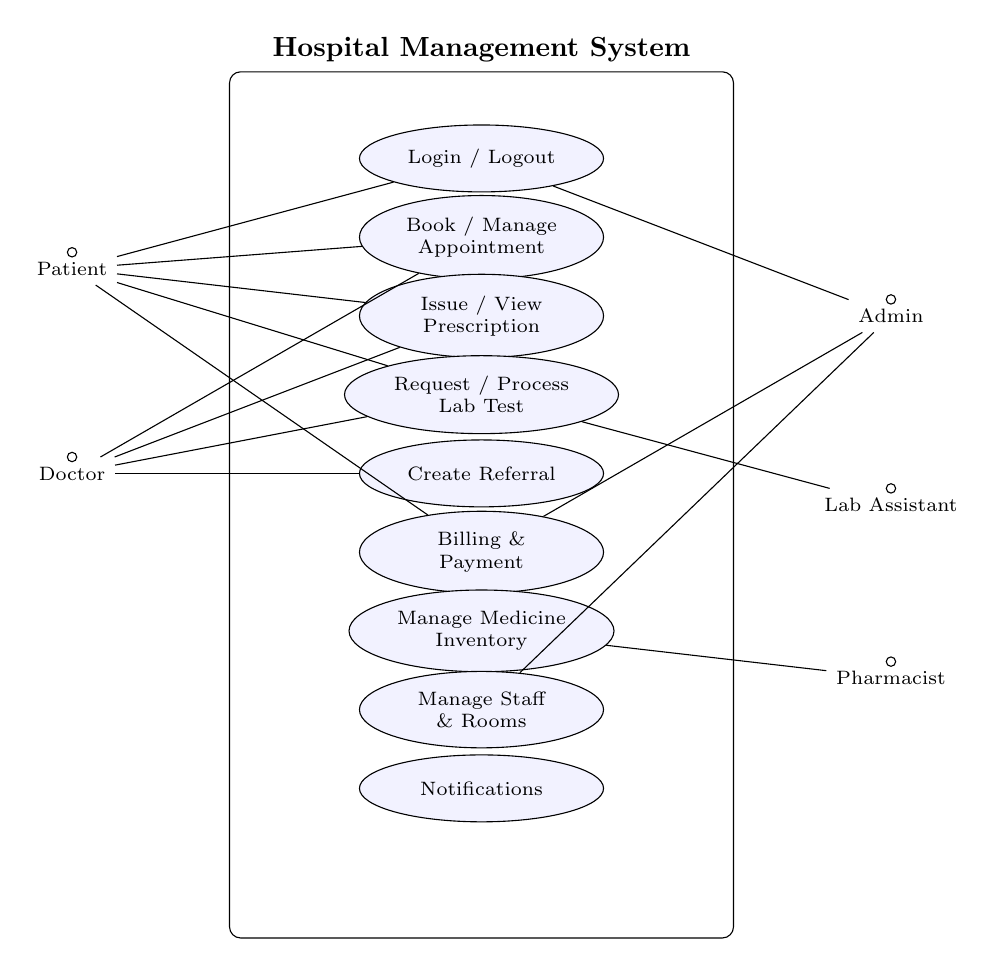
\begin{tikzpicture}[
  actor/.style={},
  usecase/.style={draw, ellipse, minimum width=3.1cm, minimum height=0.85cm, align=center, font=\scriptsize, fill=blue!5},
  node distance=0.35cm and 2.6cm]

% system boundary
\node[draw, rounded corners, minimum width=6.4cm, minimum height=11cm, label=above:{\bfseries Hospital Management System}] (sys) at (0,0) {};

% use cases (inside boundary)
\node[usecase] (login)  at (0, 4.4) {Login / Logout};
\node[usecase] (appt)   at (0, 3.4) {Book / Manage\\Appointment};
\node[usecase] (presc)  at (0, 2.4) {Issue / View\\Prescription};
\node[usecase] (lab)    at (0, 1.4) {Request / Process\\Lab Test};
\node[usecase] (refer)  at (0, 0.4) {Create Referral};
\node[usecase] (bill)   at (0,-0.6) {Billing \&\\Payment};
\node[usecase] (pharm)  at (0,-1.6) {Manage Medicine\\Inventory};
\node[usecase] (staff)  at (0,-2.6) {Manage Staff\\\& Rooms};
\node[usecase] (notif)  at (0,-3.6) {Notifications};

% actors (left)
\node[actor] (patient) at (-5.2, 3.0) {\scriptsize Patient};
\node[actor] (doctor)  at (-5.2, 0.4) {\scriptsize Doctor};

% actors (right)
\node[actor] (admin)   at (5.2, 2.4) {\scriptsize Admin};
\node[actor] (lab_a)   at (5.2, 0.0) {\scriptsize Lab Assistant};
\node[actor] (pharma)  at (5.2, -2.2){\scriptsize Pharmacist};

% draw stick-figure-ish labels
\foreach \a in {patient,doctor,admin,lab_a,pharma}{ \node[circle,draw,inner sep=1.2pt] at (\a.north) {}; }

% associations
\draw (patient) -- (login); \draw (patient) -- (appt); \draw (patient) -- (presc); \draw (patient) -- (lab); \draw (patient) -- (bill);
\draw (doctor) -- (appt); \draw (doctor) -- (presc); \draw (doctor) -- (lab); \draw (doctor) -- (refer);
\draw (admin) -- (staff); \draw (admin) -- (bill); \draw (admin) -- (login);
\draw (lab_a) -- (lab);
\draw (pharma) -- (pharm);
\end{tikzpicture}
\caption{Use Case Diagram of the Hospital Management System}
\label{fig:usecase}
\end{figure}

\paragraph{Roles.}
\begin{itemize}[leftmargin=1.4em, itemsep=1pt]
  \item \textbf{Patient} --- registers, books and manages appointments, views
        prescriptions and lab results, and pays invoices.
  \item \textbf{Doctor} --- sets availability, consults patients, issues prescriptions,
        orders lab tests, and refers patients.
  \item \textbf{Lab Assistant} --- processes lab-test requests and records results.
  \item \textbf{Pharmacist} --- manages the location-aware medicine inventory.
  \item \textbf{Administrator} --- manages staff accounts, rooms, billing, and
        system-wide records.
\end{itemize}

\subsection{Architectural Design}
The Hospital Management System is designed using a \textbf{layered architecture}, which
separates the system into distinct layers, each with specific responsibilities. This
modular approach improves maintainability, scalability, and readability.

\paragraph{Presentation Layer.} Implemented using React with Vite, this layer manages
the user interface and experience. It includes role-specific pages (Login, Register,
and the Patient, Doctor, Admin, Lab, and Pharmacist dashboards) and shared components
such as \texttt{DashboardLayout}, \texttt{ProtectedRoute}, \texttt{DataTable},
\texttt{NotificationBell}, and an authentication context. It communicates with the
backend through Axios HTTP requests, attaching the access token and transparently
refreshing it when it expires.

\paragraph{Application Layer.} Built with Express.js, this layer contains the business
logic and middleware. Its key components include:
\begin{itemize}[leftmargin=1.4em, itemsep=1pt]
  \item \textbf{Controllers:} \texttt{authController}, \texttt{appointmentController},
        \texttt{availabilityController}, \texttt{prescriptionController},
        \texttt{labController}, \texttt{referralController}, \texttt{invoiceController},
        \texttt{notificationController}, \texttt{medicineController}, and
        \texttt{staffController}.
  \item \textbf{Routes:} one router per resource, mounted under \texttt{/api/v1/hms}.
  \item \textbf{Middleware:} \texttt{authenticate} and \texttt{authorise} (JWT
        verification and role checks), \texttt{rateLimit}, and centralised error
        handling.
  \item \textbf{Services:} \texttt{tokenService}, \texttt{contactService},
        \texttt{notificationService}, \texttt{availabilityService},
        \texttt{mailer} (Nodemailer), and \texttt{sms} (Twilio).
\end{itemize}

\paragraph{Data Layer.} The data layer consists of MySQL with Sequelize models defining
schemas, associations, and constraints. It manages persistent data for users, patients,
staff, appointments, availability, prescriptions, lab tests, referrals, invoices,
notifications, medicines, and verification tokens, enforcing referential integrity and
cascade rules.

\begin{figure}[htbp]
\centering
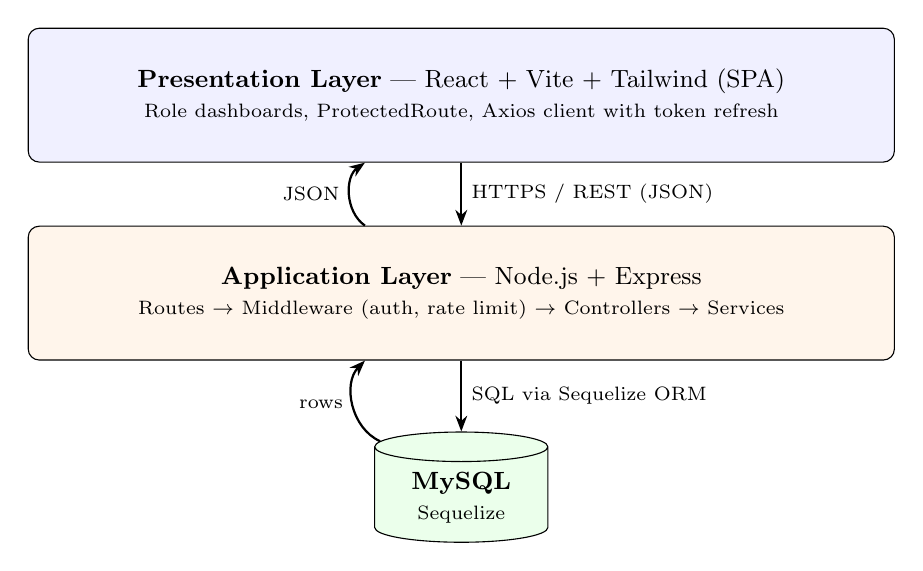
\begin{tikzpicture}[font=\small, node distance=1.0cm,
  layer/.style={draw, rounded corners, minimum width=11cm, minimum height=1.7cm, align=center},
  db/.style={draw, cylinder, shape border rotate=90, aspect=0.25, minimum width=2.2cm, minimum height=1.4cm, align=center, fill=green!8}]
\node[layer, fill=blue!6] (pres) {\textbf{Presentation Layer} --- React + Vite + Tailwind (SPA)\\
  \scriptsize Role dashboards, ProtectedRoute, Axios client with token refresh};
\node[layer, fill=orange!8, below=0.8cm of pres] (app) {\textbf{Application Layer} --- Node.js + Express\\
  \scriptsize Routes $\rightarrow$ Middleware (auth, rate limit) $\rightarrow$ Controllers $\rightarrow$ Services};
\node[db, below=0.9cm of app] (data) {\textbf{MySQL}\\\scriptsize Sequelize};
\draw[arrow] (pres) -- node[right]{\scriptsize HTTPS / REST (JSON)} (app);
\draw[arrow] (app) -- node[right]{\scriptsize SQL via Sequelize ORM} (data);
\draw[arrow] (data) to[bend left=55] node[left]{\scriptsize rows} (app);
\draw[arrow] (app) to[bend left=55] node[left]{\scriptsize JSON} (pres);
\end{tikzpicture}
\caption{Client--Server Layered Architecture of the Hospital Management System}
\label{fig:arch}
\end{figure}

\subsection{Module or Component Design}
The system is divided into several modules, each responsible for specific
functionality. This modular structure improves organisation, reusability, and
maintainability.
\begin{itemize}[leftmargin=1.4em]
  \item \textbf{Authentication Module:} Handles registration, login, logout, token
        refresh, password reset, and email verification, backed by hashed credentials
        and rotating refresh tokens.
  \item \textbf{Appointment Module:} Manages doctor availability, one-off time off, and
        the booking lifecycle, preventing conflicts against existing bookings.
  \item \textbf{Clinical Module:} Covers prescriptions, laboratory tests, and referrals,
        linking doctors, patients, and lab assistants.
  \item \textbf{Billing Module:} Manages invoices, line items, payments, and status.
  \item \textbf{Pharmacy Module:} Manages the location-aware medicine catalogue and
        stock adjustments.
  \item \textbf{Notification Module:} Creates in-app notifications and dispatches email
        and SMS through the mailer and SMS services.
  \item \textbf{Administration Module:} Manages staff accounts, rooms, and user status.
\end{itemize}
Each module functions independently but interacts through the RESTful APIs, so the
system can be maintained, upgraded, or extended with minimal coupling.

\subsection{Database or Data Design}
The Hospital Management System uses \textbf{MySQL} as the primary database and
\textbf{Sequelize} for defining models and relationships. Unlike a document store, the
schema is normalised into related tables with enforced foreign keys and cascade rules.
The principal entities are:
\begin{itemize}[leftmargin=1.4em, itemsep=1pt]
  \item \textbf{User} --- credentials, role, active status, and refresh-token version;
        the root of authentication.
  \item \textbf{Patient} / \textbf{StaffProfile} --- role-specific profile data linked
        one-to-one to a User.
  \item \textbf{Appointment}, \textbf{DoctorAvailability}, \textbf{DoctorTimeOff} ---
        scheduling data linking patients and doctors.
  \item \textbf{Prescription}, \textbf{LabTest}, \textbf{Referral} --- clinical records.
  \item \textbf{Invoice} --- billing linked to a patient.
  \item \textbf{Medicine} --- the pharmacy catalogue with location and stock.
  \item \textbf{Notification}, \textbf{VerificationToken} --- alerts and single-use
        security tokens.
\end{itemize}

\begin{figure}[htbp]
\centering
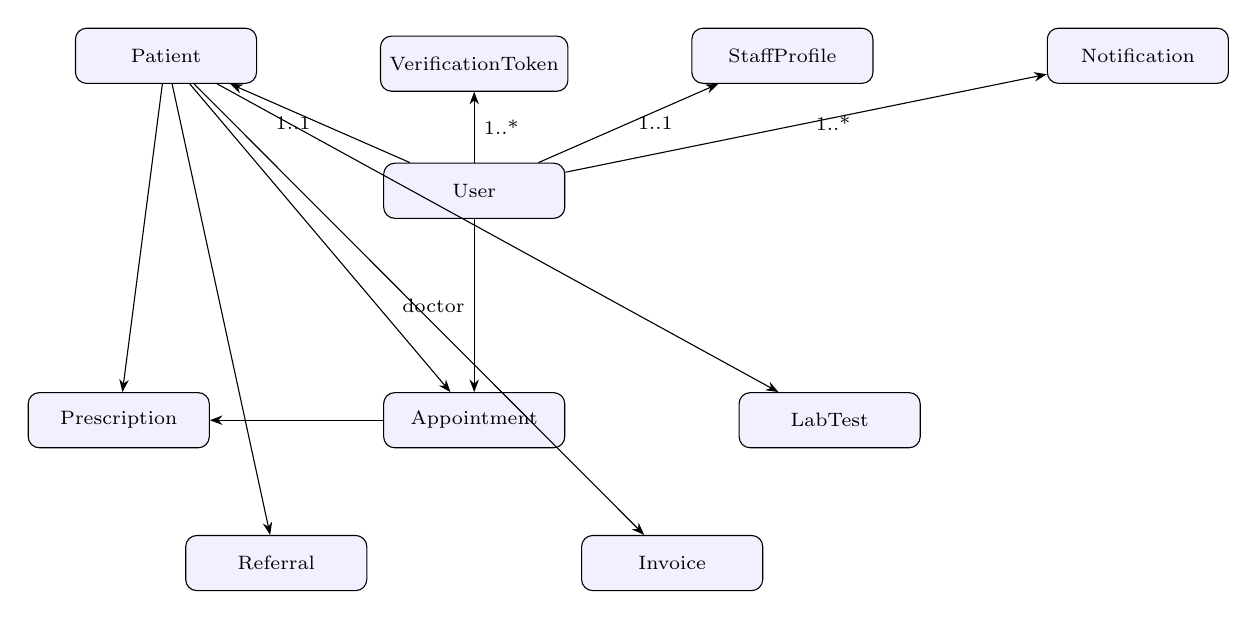
\begin{tikzpicture}[font=\scriptsize,
  ent/.style={draw, rounded corners, fill=blue!6, minimum width=2.3cm, minimum height=0.7cm, align=center},
  rel/.style={-{Stealth[length=1.6mm]}}]
\node[ent] (user) {User};
\node[ent, above left=1.0cm and 1.6cm of user] (patient) {Patient};
\node[ent, above right=1.0cm and 1.6cm of user] (staff) {StaffProfile};
\node[ent, below=2.2cm of user] (appt) {Appointment};
\node[ent, left=2.2cm of appt] (presc) {Prescription};
\node[ent, right=2.2cm of appt] (lab) {LabTest};
\node[ent, below left=1.1cm and 0.2cm of appt] (refer) {Referral};
\node[ent, below right=1.1cm and 0.2cm of appt] (invoice) {Invoice};
\node[ent, right=2.2cm of staff] (notif) {Notification};
\node[ent, above=0.9cm of user] (vtoken) {VerificationToken};

\draw[rel] (user) -- node[left]{1..1} (patient);
\draw[rel] (user) -- node[right]{1..1} (staff);
\draw[rel] (user) -- node[right]{1..*} (vtoken);
\draw[rel] (user) -- node[right]{1..*} (notif);
\draw[rel] (patient) -- (appt);
\draw[rel] (user) -- node[left]{doctor} (appt);
\draw[rel] (patient) -- (presc);
\draw[rel] (patient) -- (lab);
\draw[rel] (patient) -- (refer);
\draw[rel] (patient) -- (invoice);
\draw[rel] (appt) -- (presc);
\end{tikzpicture}
\caption{Entity--Relationship overview (principal entities and relationships)}
\label{fig:er}
\end{figure}

\section{Implementation Details}

\subsection{Software Implementation}
The system is implemented as a full-stack web application with a clear separation
between the React frontend and the Express backend, communicating over RESTful APIs.

\paragraph{Frontend.} React (with Vite) builds a responsive single-page application
styled with Tailwind CSS. Axios handles API communication, attaching the JWT access
token to each request and transparently refreshing it on expiry. Routing is handled by
React Router, with a \texttt{ProtectedRoute} component restricting each dashboard to its
allowed roles. Authentication state is held in a React context, and toast notifications
provide user feedback.

\paragraph{Backend.} Node.js with Express implements the RESTful API in a modular
structure with separate routes, controllers, middleware, and services. Controllers
encapsulate business logic such as booking appointments, issuing prescriptions,
processing lab tests, and recording payments. Middleware enforces authentication,
role-based authorisation, and rate limiting, and centralised error handling returns
consistent responses without leaking internal details.

\paragraph{Database.} MySQL stores all persistent data, with Sequelize models defining
schemas, validations, associations, and cascade rules. The use of an ORM provides schema
consistency, parameterised queries that mitigate SQL injection, and readable
association-based data access.

\paragraph{Security.} Passwords are hashed with bcrypt. JWT access tokens are
short-lived, while refresh tokens are stored in HTTP-only cookies and versioned so they
can be revoked (for example, after a password reset). Password-reset and
email-verification tokens are single-use and stored only as SHA-256 hashes, and the
mail-sending endpoints are rate limited to resist abuse and account enumeration.

\subsection{Hardware Implementation}
The system does not require specialised hardware and runs on standard computing devices.
During development and testing it was implemented and evaluated on a personal computer
with a dual-core processor, at least 4 GB of RAM, and a local MySQL server. The backend
runs on the Node.js runtime, while the frontend runs in a modern web browser, making the
system portable across personal computers, institutional servers, and cloud hosts.

\section{Algorithms and Flowcharts}
This section describes the key algorithms used in the system and the logical flow of
major operations. These ensure secure authentication, conflict-free scheduling, and
proper role-based access control.

\begin{algorithm}[htbp]
\caption{User Login (JWT)}
\begin{algorithmic}[1]
\State \textbf{Start}
\State User submits identifier, password, and role
\State Validate that all fields are present
\State Look up the user by identifier; verify the role matches and the account is active
\State Compare the submitted password with the stored bcrypt hash
\If{credentials are valid}
  \State Sign a short-lived \emph{access token} and a \emph{refresh token} (with token version)
  \State Set the refresh token as an HTTP-only cookie
  \State Return the access token and user profile
\Else
  \State Return a generic ``Invalid credentials'' error
\EndIf
\State \textbf{End}
\end{algorithmic}
\end{algorithm}

\begin{algorithm}[htbp]
\caption{Access-Token Refresh with Rotation}
\begin{algorithmic}[1]
\State \textbf{Start}
\State Read the refresh token from the HTTP-only cookie
\State Verify the token signature and expiry
\State Look up the user and compare the token version
\If{token is valid and version matches}
  \State Issue a new access token
\Else
  \State Reject the request and require re-authentication
\EndIf
\State \textbf{End}
\end{algorithmic}
\end{algorithm}

\begin{algorithm}[htbp]
\caption{Password Reset}
\begin{algorithmic}[1]
\State \textbf{Start}
\State User requests a reset with their identifier
\State Respond identically whether or not the account exists (no enumeration)
\If{account exists and is active}
  \State Generate a random token; store only its SHA-256 hash with an expiry
  \State Email the raw token as a reset link
\EndIf
\State On reset: validate the token hash and expiry; if valid, hash the new password,
       save it, and \emph{increment the refresh-token version} to revoke all sessions
\State \textbf{End}
\end{algorithmic}
\end{algorithm}

\begin{algorithm}[htbp]
\caption{Appointment Booking}
\begin{algorithmic}[1]
\State \textbf{Start}
\State Patient selects a doctor, date, and time slot
\State Verify authentication and patient role
\State Check the doctor's weekly availability and one-off time off for that slot
\State Check for an existing appointment conflicting with the slot
\If{slot is available and free}
  \State Create the appointment with status \emph{pending}
  \State Notify the doctor (in-app and email)
\Else
  \State Return an error indicating the slot is unavailable
\EndIf
\State \textbf{End}
\end{algorithmic}
\end{algorithm}

\begin{algorithm}[htbp]
\caption{Role-Based Access Control}
\begin{algorithmic}[1]
\State \textbf{Start}
\State User sends a request to a protected route with an access token
\State Verify the JWT and load the active user
\State Extract the user's role
\If{role is permitted for the route}
  \State Allow the request to proceed
\Else
  \State Deny access and return an authorisation error
\EndIf
\State \textbf{End}
\end{algorithmic}
\end{algorithm}

\paragraph{Flowchart --- Appointment Booking.}
Figure~\ref{fig:flow-appt} illustrates the booking process from slot selection through
availability checking to record creation and notification.

\begin{figure}[htbp]
\centering
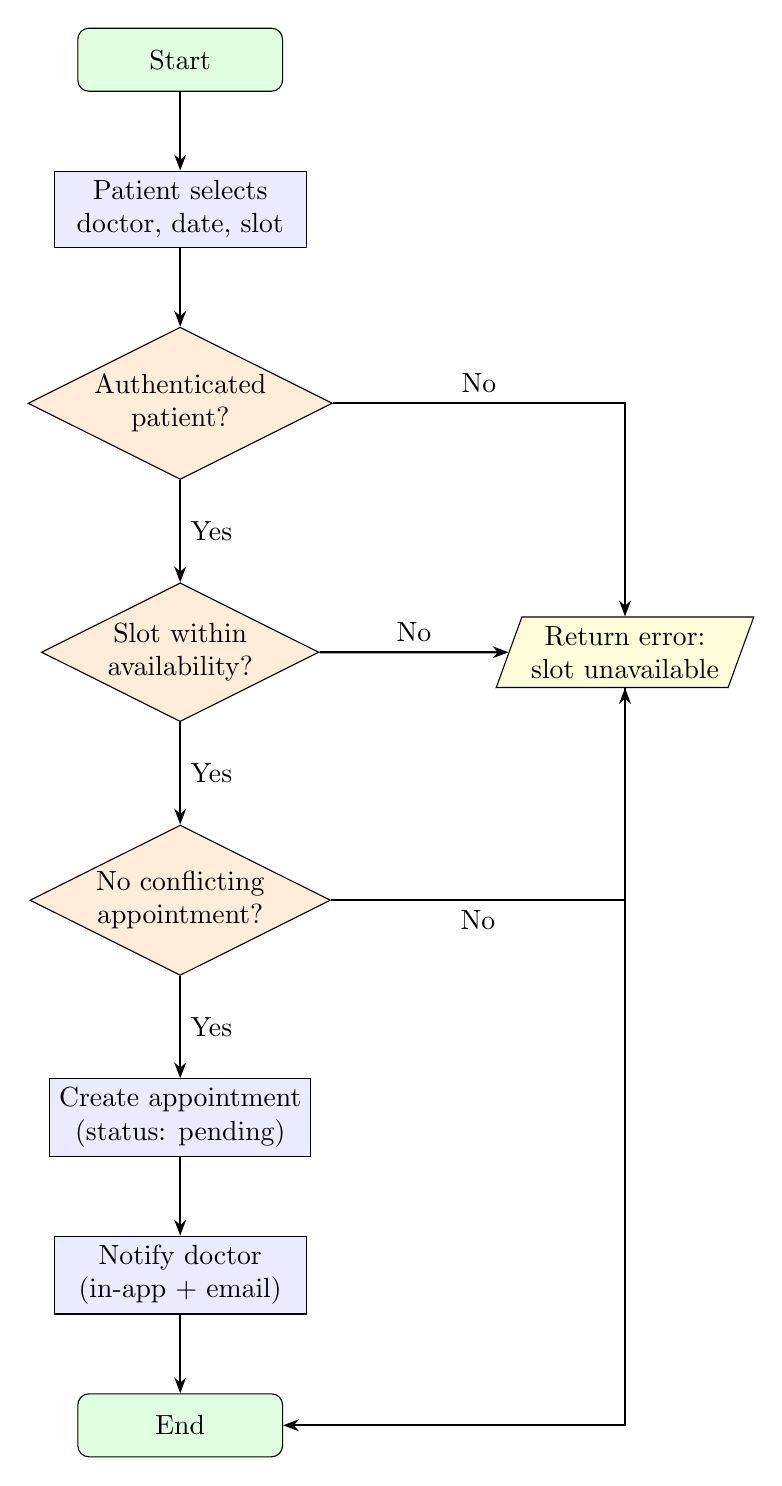
\begin{tikzpicture}[node distance=1.0cm and 1.4cm]
\node[startstop] (start) {Start};
\node[process, below=of start] (select) {Patient selects\\doctor, date, slot};
\node[decision, below=of select] (auth) {Authenticated\\patient?};
\node[decision, below=1.3cm of auth] (avail) {Slot within\\availability?};
\node[decision, below=1.3cm of avail] (free) {No conflicting\\appointment?};
\node[process, below=1.3cm of free] (create) {Create appointment\\(status: pending)};
\node[process, below=of create] (notify) {Notify doctor\\(in-app + email)};
\node[startstop, below=of notify] (end) {End};
\node[io, right=2.4cm of avail] (err) {Return error:\\slot unavailable};

\draw[arrow] (start) -- (select);
\draw[arrow] (select) -- (auth);
\draw[arrow] (auth) -- node[right]{Yes} (avail);
\draw[arrow] (avail) -- node[right]{Yes} (free);
\draw[arrow] (free) -- node[right]{Yes} (create);
\draw[arrow] (create) -- (notify);
\draw[arrow] (notify) -- (end);
\draw[arrow] (auth) -| node[near start, above]{No} (err);
\draw[arrow] (avail) -- node[above]{No} (err);
\draw[arrow] (free) -| node[near start, below]{No} (err);
\draw[arrow] (err) |- (end);
\end{tikzpicture}
\caption{Appointment Booking Flowchart}
\label{fig:flow-appt}
\end{figure}

\paragraph{Flowchart --- Authentication.}
Figure~\ref{fig:flow-auth} shows the login process: credential validation, token
generation, and error handling.

\begin{figure}[htbp]
\centering
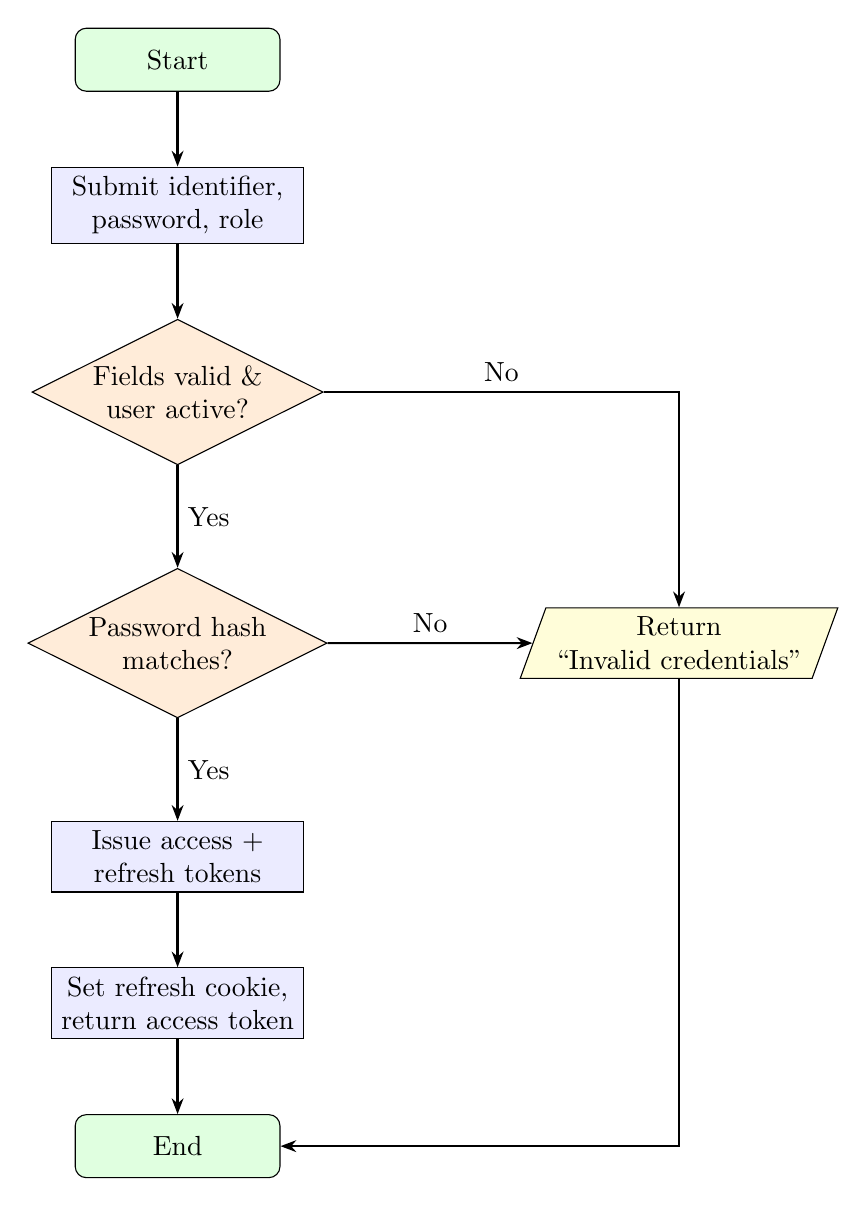
\begin{tikzpicture}[node distance=0.95cm and 1.4cm]
\node[startstop] (s) {Start};
\node[process, below=of s] (sub) {Submit identifier,\\password, role};
\node[decision, below=of sub] (val) {Fields valid \&\\user active?};
\node[decision, below=1.3cm of val] (pw) {Password hash\\matches?};
\node[process, below=1.3cm of pw] (tok) {Issue access +\\refresh tokens};
\node[process, below=of tok] (cook) {Set refresh cookie,\\return access token};
\node[startstop, below=of cook] (e) {End};
\node[io, right=2.6cm of pw] (err) {Return\\``Invalid credentials''};
\draw[arrow] (s)--(sub); \draw[arrow] (sub)--(val);
\draw[arrow] (val)-- node[right]{Yes}(pw);
\draw[arrow] (pw)-- node[right]{Yes}(tok);
\draw[arrow] (tok)--(cook); \draw[arrow] (cook)--(e);
\draw[arrow] (val)-| node[near start,above]{No}(err);
\draw[arrow] (pw)-- node[above]{No}(err);
\draw[arrow] (err)|-(e);
\end{tikzpicture}
\caption{User Authentication Flowchart}
\label{fig:flow-auth}
\end{figure}

\section{Tools and Technologies Used}
This project uses modern web-development tools and technologies to ensure efficiency,
scalability, and maintainability, supporting secure, responsive, and modular design.

\begin{table}[htbp]
\centering
\renewcommand{\arraystretch}{1.3}
\begin{tabular}{@{}p{4.2cm} p{9cm}@{}}
\toprule
\textbf{Layer / Component} & \textbf{Technologies / Tools Used} \\
\midrule
Frontend & React, Vite, Tailwind CSS, Axios, React Router, React Toastify \\
Backend & Node.js, Express.js \\
Database & MySQL, Sequelize (ORM) \\
Authentication & JSON Web Tokens (JWT), bcrypt, HTTP-only cookies \\
Notifications & Nodemailer (email), Twilio (SMS) \\
Development Tools & Visual Studio Code, Git, GitHub, Nodemon, ESLint \\
\bottomrule
\end{tabular}
\caption{Technologies Used in the Hospital Management System}
\label{tab:tech}
\end{table}

% ===========================================================================
% CHAPTER 4 — RESULTS AND DISCUSSION
% ===========================================================================
\chapter{Results and Discussion}
This chapter presents the results of the implemented Hospital Management System,
analyses its behaviour, and compares the outcomes with the objectives stated in
Chapter~1. It also discusses the challenges and limitations encountered during
development.

\section{Implemented Features}
The system successfully implements the following key features.

\paragraph{Secure Login and Authentication.} Users log in through a role-aware form.
Authentication is backed by bcrypt-hashed passwords and JWT access tokens, with refresh
tokens rotated through HTTP-only cookies. Password-reset and email-verification flows are
also provided.
\rfig{pica/log.png}{Login page --- role-aware, secure sign-in}{fig:login}
\paragraph{Password Reset and Email Verification.} A ``Forgot password'' flow issues a
single-use, hash-stored reset link by email, and new accounts receive a verification
link. Where a mail server is not configured, messages are logged to the server console,
so the flows remain testable in development.
\screenshot{Forgot-password page (screenshot to be added).}

\paragraph{Role-Based Dashboards.} Each of the five roles has a distinct dashboard.
The \emph{patient} dashboard shows appointments, prescriptions, lab tests, and billing;
the \emph{doctor} dashboard shows the appointment queue, schedule, patients, and
referrals; the \emph{admin} dashboard shows users, staff, billing, lab requests, and
room management; the \emph{lab} and \emph{pharmacist} portals show their respective
queues and inventory.
\rfig{pica/patient.png}{Patient dashboard}{fig:patient}
\rfig{pica/doctor.png}{Doctor dashboard}{fig:doctor}
\rfig{pica/admin.png}{Admin dashboard}{fig:admin}

\paragraph{Appointment Management.} Patients book appointments against a doctor's
declared availability, with conflict checking; appointments move through a
pending/confirmed/cancelled/completed workflow.
\screenshot{Appointment booking and management (screenshot to be added).}

\paragraph{Prescriptions, Lab Tests, and Referrals.} Doctors issue prescriptions,
order lab tests, and refer patients; lab assistants process test requests and record
results, which patients can then view.
\rfig{pica/lab.png}{Lab Assistant portal --- test-request queue and results}{fig:lab}

\paragraph{Billing and Pharmacy Inventory.} Administrators issue invoices and record
payments; pharmacists manage a location-aware medicine catalogue with stock levels,
reorder thresholds, and expiry.
\rfig{pica/pharm.png}{Pharmacist portal --- location-aware medicine inventory}{fig:pharm}

\paragraph{Notifications.} In-application notifications are created for appointments,
prescriptions, lab tests, referrals, and invoices, and are mirrored to the user's email
(and optionally SMS), so patients are informed without logging in.

\section{Results and Performance Analysis}
The system was tested on a standard personal computer with a local MySQL server. The
backend started successfully, established a database connection, and synchronised all
thirteen models; the frontend built and served without errors; and the REST endpoints
returned correct responses for authentication, booking, and billing flows. Typical API
responses completed well within the 2--3 second target under normal single-user load.

\section{Comparison with Project Objectives}
The implemented system meets the objectives stated in Chapter~1:
\begin{itemize}[leftmargin=1.4em]
  \item \textbf{Web-Based Design:} a full-stack architecture (React + Node.js/Express +
        MySQL) is in place.
  \item \textbf{Secure Authentication:} JWT with refresh-token rotation, password reset,
        and email verification secure access, with five-way role-based control.
  \item \textbf{Workflow Automation:} appointments, prescriptions, lab tests, referrals,
        billing, and pharmacy inventory are all implemented.
  \item \textbf{Multi-Channel Notifications:} in-app, email, and SMS notifications keep
        users informed.
  \item \textbf{Usability:} responsive, role-specific dashboards provide an intuitive
        interface.
\end{itemize}

\section{Challenges and Limitations}
\begin{itemize}[leftmargin=1.4em]
  \item \textbf{Schema Evolution:} during development the schema is synchronised
        automatically; a production deployment would need managed migrations.
  \item \textbf{Concurrency:} some multi-step operations (for example, recording
        payments) would benefit from database transactions to remain fully atomic under
        concurrent load.
  \item \textbf{External Delivery:} real email/SMS delivery depends on third-party
        providers being configured; without them the system falls back to console
        logging.
  \item \textbf{No Mobile Application:} the system is currently web-only.
  \item \textbf{Automated Testing:} the current version relies on manual verification
        rather than an automated test suite.
\end{itemize}

\section{Discussion}
The Hospital Management System demonstrates effective integration of frontend and
backend technologies. Axios and RESTful APIs provide smooth communication between the
React frontend and the Express backend; JWT-based authentication with refresh-token
rotation provides secure, revocable access; the layered architecture separates
presentation, application, and data concerns; and the normalised MySQL schema enforces
referential integrity across clinical and administrative records. The modular design
makes it straightforward to add further features.

\section{Summary}
The implemented system achieves its primary objectives of secure authentication,
role-based access, automated hospital workflows, and multi-channel notification. While
some limitations remain, the system provides a solid foundation for future enhancement
and a practical tool for managing hospital operations.

% ===========================================================================
% CHAPTER 5 — CONCLUSION AND FUTURE WORKS
% ===========================================================================
\chapter{Conclusion and Future Works}

\section{Conclusion}
The Hospital Management System developed in this project successfully fulfils the
primary objectives outlined in Chapter~1 by providing a secure, web-based platform for
managing hospital operations across five distinct roles. The system implements JWT-based
authentication with refresh-token rotation to ensure secure, revocable access and
enforces role-based authorisation, while dedicated dashboards for patients, doctors,
administrators, lab assistants, and pharmacists enhance usability. Patients can book and
manage appointments, view prescriptions and lab results, and settle bills; doctors
manage availability, prescriptions, lab orders, and referrals; and administrators manage
staff, billing, and rooms. Appointments, prescriptions, lab tests, referrals, and
invoices are handled with automatic status updates and notifications delivered both
in-app and by email. The frontend, built with React and Tailwind CSS, offers a
responsive and user-friendly interface, while the modular client--server architecture
combined with MySQL and Sequelize ensures maintainability and flexibility for future
expansion. Overall, the project demonstrates the effective integration of modern
frontend and backend technologies, secure authentication, and reliable relational data
management.

\section{Limitations}
While the system is fully functional, a few limitations exist in the current version:
\begin{itemize}[leftmargin=1.4em]
  \item \textbf{Managed Migrations:} the schema is auto-synchronised in development
        rather than versioned through migrations.
  \item \textbf{Transactions:} some multi-step flows are not yet fully transactional.
  \item \textbf{Provider Dependency:} outbound email and SMS require external providers
        to be configured.
  \item \textbf{Mobile Support:} the system is currently web-only.
\end{itemize}

\section{Future Works}
The modular and scalable architecture allows for multiple future enhancements:
\begin{itemize}[leftmargin=1.4em]
  \item \textbf{Database Migrations and Transactions:} adopt versioned migrations and
        wrap critical flows (payments, booking) in transactions.
  \item \textbf{Automated Testing and CI:} add unit and integration tests with
        continuous integration.
  \item \textbf{Advanced Scheduling and Analytics:} smarter slot allocation, queue
        management, and dashboards tracking hospital usage and trends.
  \item \textbf{Mobile Application:} a companion app for Android and iOS.
  \item \textbf{Inpatient and Pharmacy Extensions:} ward/bed management and automatic
        stock deduction on dispensing.
  \item \textbf{Audit Logging and Compliance:} record access to medical data to support
        privacy and compliance requirements.
\end{itemize}
The system is designed with future scalability in mind, allowing it to evolve into a
comprehensive hospital management solution suitable for modern healthcare institutions.

% ===========================================================================
% REFERENCES
% ===========================================================================
\begin{thebibliography}{99}
\addcontentsline{toc}{chapter}{References}
\bibitem{react} React: Official documentation. \url{https://react.dev/}. Accessed \today.
\bibitem{node} Node.js: Official documentation. \url{https://nodejs.org/en/docs/}. Accessed \today.
\bibitem{express} Express.js: Official guide. \url{https://expressjs.com/}. Accessed \today.
\bibitem{mysql} MySQL: Official documentation. \url{https://dev.mysql.com/doc/}. Accessed \today.
\bibitem{sequelize} Sequelize: ORM documentation. \url{https://sequelize.org/docs/v6/}. Accessed \today.
\bibitem{jwt} JSON Web Tokens: Introduction. \url{https://jwt.io/introduction/}. Accessed \today.
\bibitem{tailwind} Tailwind CSS: Documentation. \url{https://tailwindcss.com/docs}. Accessed \today.
\bibitem{axios} Axios: Promise-based HTTP client. \url{https://axios-http.com/docs/intro}. Accessed \today.
\bibitem{nodemailer} Nodemailer: Documentation. \url{https://nodemailer.com/}. Accessed \today.
\bibitem{openmrs} OpenMRS: Open-source medical record platform. \url{https://openmrs.org/}. Accessed \today.
\end{thebibliography}

% ===========================================================================
% APPENDIX
% ===========================================================================
\appendix
\chapter*{Appendix-A}
\addcontentsline{toc}{chapter}{Appendix-A}

\section*{A.1\quad Source Code Snippets}

\subsection*{A.1.1\quad Backend: User Model (User.js)}
The following snippet shows the Sequelize model for the \texttt{users} table, including
the role enumeration, refresh-token version used for session revocation, and the
email-verification timestamp.
\begin{lstlisting}[language=Java]
const User = sequelize.define("User", {
  id: { type: DataTypes.UUID, defaultValue: DataTypes.UUIDV4, primaryKey: true },
  identifier: { type: DataTypes.STRING(100), allowNull: false, unique: true },
  password_hash: { type: DataTypes.STRING(255), allowNull: false },
  role: {
    type: DataTypes.ENUM("patient","doctor","pharmacist","lab_assistant","admin"),
    allowNull: false,
  },
  refresh_token_version: { type: DataTypes.INTEGER, defaultValue: 0 },
  email_verified_at: { type: DataTypes.DATE, allowNull: true },
  is_active: { type: DataTypes.BOOLEAN, defaultValue: true },
}, { tableName: "users", timestamps: true });
\end{lstlisting}

\subsection*{A.1.2\quad Backend: Role-Based Access Middleware (auth.js)}
This middleware verifies the JWT and restricts a route to specific roles.
\begin{lstlisting}[language=Java]
export const authenticate = async (req, res, next) => {
  const authHeader = req.headers.authorization;
  if (!authHeader?.startsWith("Bearer"))
    return res.status(401).json({ message: "No token provided" });
  const decoded = verifyAccessToken(authHeader.split(" ")[1]);
  const user = await User.findByPk(decoded.id,
    { attributes: { exclude: ["password_hash"] } });
  if (!user || !user.is_active)
    return res.status(401).json({ message: "User not found or inactive" });
  req.user = user;
  next();
};

export const authorise = (...roles) => (req, res, next) => {
  if (!roles.includes(req.user?.role))
    return res.status(403).json({ message: "Access denied" });
  next();
};
\end{lstlisting}

\section*{A.2\quad API Endpoints Summary}
The table below summarises the main API endpoints (base path \texttt{/api/v1/hms}).
\begin{table}[htbp]
\centering
\renewcommand{\arraystretch}{1.25}
\begin{tabular}{@{}p{5.6cm} p{1.8cm} p{5.4cm}@{}}
\toprule
\textbf{Endpoint} & \textbf{Method} & \textbf{Description} \\
\midrule
\texttt{/register} & POST & Register a new patient \\
\texttt{/login} & POST & Log in an existing user \\
\texttt{/refresh} & POST & Refresh the access token \\
\texttt{/forgot-password} & POST & Request a password-reset link \\
\texttt{/reset-password} & POST & Set a new password from a token \\
\texttt{/verify-email} & POST & Verify an email address \\
\texttt{/staff} & POST & Create a staff account (admin) \\
\texttt{/appointments} & POST & Book an appointment \\
\texttt{/prescriptions} & POST & Issue a prescription \\
\texttt{/labs} & POST & Request a lab test \\
\texttt{/invoices} & POST & Create an invoice (admin) \\
\texttt{/medicines} & GET & List the medicine catalogue \\
\bottomrule
\end{tabular}
\caption{Main API Endpoints of the HMS}
\label{tab:api}
\end{table}

\section*{A.3\quad Configuration Files}
Example environment variables (\texttt{.env}) storing sensitive configuration such as
the database connection, JWT secrets, and optional mail/SMS providers:
\begin{lstlisting}
PORT=8000
NODE_ENV=development
CLIENT_URL=http://localhost:5173

DB_HOST=localhost
DB_PORT=3306
DB_NAME=hms_db
DB_USER=root
DB_PASSWORD=your_password

JWT_ACCESS_SECRET=your_access_secret
JWT_REFRESH_SECRET=your_refresh_secret

# Optional: outbound email (falls back to console when unset)
MAIL_HOST=
MAIL_PORT=587
MAIL_FROM=no-reply@dhulikhel-hms.local

# Optional: outbound SMS (falls back to console when unset)
TWILIO_ACCOUNT_SID=
TWILIO_AUTH_TOKEN=
TWILIO_FROM_NUMBER=
\end{lstlisting}

\section*{A.4\quad Project Timeline: Gantt Chart}
The Gantt chart in Figure~\ref{fig:gantt} illustrates the timeline of major tasks and
milestones for the HMS project over eight weeks.

\begin{figure}[htbp]
\centering
\begin{ganttchart}[
  hgrid, vgrid, x unit=1.05cm, y unit title=0.6cm, y unit chart=0.55cm,
  bar/.style={fill=blue!30}, title height=1, bar height=0.5,
  milestone/.style={fill=orange!70}]{1}{8}
\gantttitle{Project Timeline (Weeks)}{8} \\
\gantttitlelist{1,...,8}{1} \\
\ganttbar{Planning \& Analysis}{1}{2} \\
\ganttbar{Design}{2}{3} \\
\ganttbar{Development}{3}{6} \\
\ganttbar{Testing}{6}{7} \\
\ganttbar{Deployment}{7}{8} \\
\ganttmilestone{Requirements Complete}{2} \\
\ganttmilestone{Design Complete}{3} \\
\ganttmilestone{Development Complete}{6} \\
\ganttmilestone{Project Complete}{8}
\end{ganttchart}
\caption{Eight-Week Project Timeline --- Major Phases}
\label{fig:gantt}
\end{figure}

\end{document}
